\documentclass[12pt, a4paper]{article}

% Required Packages
\usepackage{graphicx}
\usepackage{geometry}
\usepackage{hyperref}
\usepackage{float}
\usepackage{caption}

% Page Geometry Setup
\geometry{
    top=2.5cm,
    bottom=2.5cm,
    left=2.5cm,
    right=2.5cm
}

\begin{document}

\begin{titlepage}
    \centering
    \vspace*{2cm}
    
    {\Huge \textbf{UML Diagrams}}\\[0.5cm]
    {\Large \textbf{NexusNotes}}\\[0.5cm]
    {\large Centralized Academic Resource Platform}\\[2cm]
    
    \textbf{Project Team: Code Club}\\[0.5cm]
    Ramasani Adi Pranav -- 24CSB0A57\\
    Syed Mohammad Sami -- 24CSB0A77\\
    Janapala Harsha Vardhan Reddy -- 24CSB0A28\\[2cm]
    
    \vfill
    {\large \textbf{Version 1.0}}\\
    {\large \today}
    
\end{titlepage}

\tableofcontents
\newpage


\newpage

\section{Introduction}

This document provides a comprehensive overview of the Unified Modeling Language (UML) diagrams for the Nexus Notes platform. Nexus Notes is a centralized academic knowledge platform that integrates students, faculty, and academic resources into a unified digital ecosystem. The following sections detail the Use Case, Sequence, Collaboration, and Activity diagrams that map out the system's architecture and user interactions.

\section{Use Case Diagram}

The Use Case Diagram provides a high-level overview of the interactions between the system's actors and its core functionalities.

\begin{figure}[H]
    \centering
    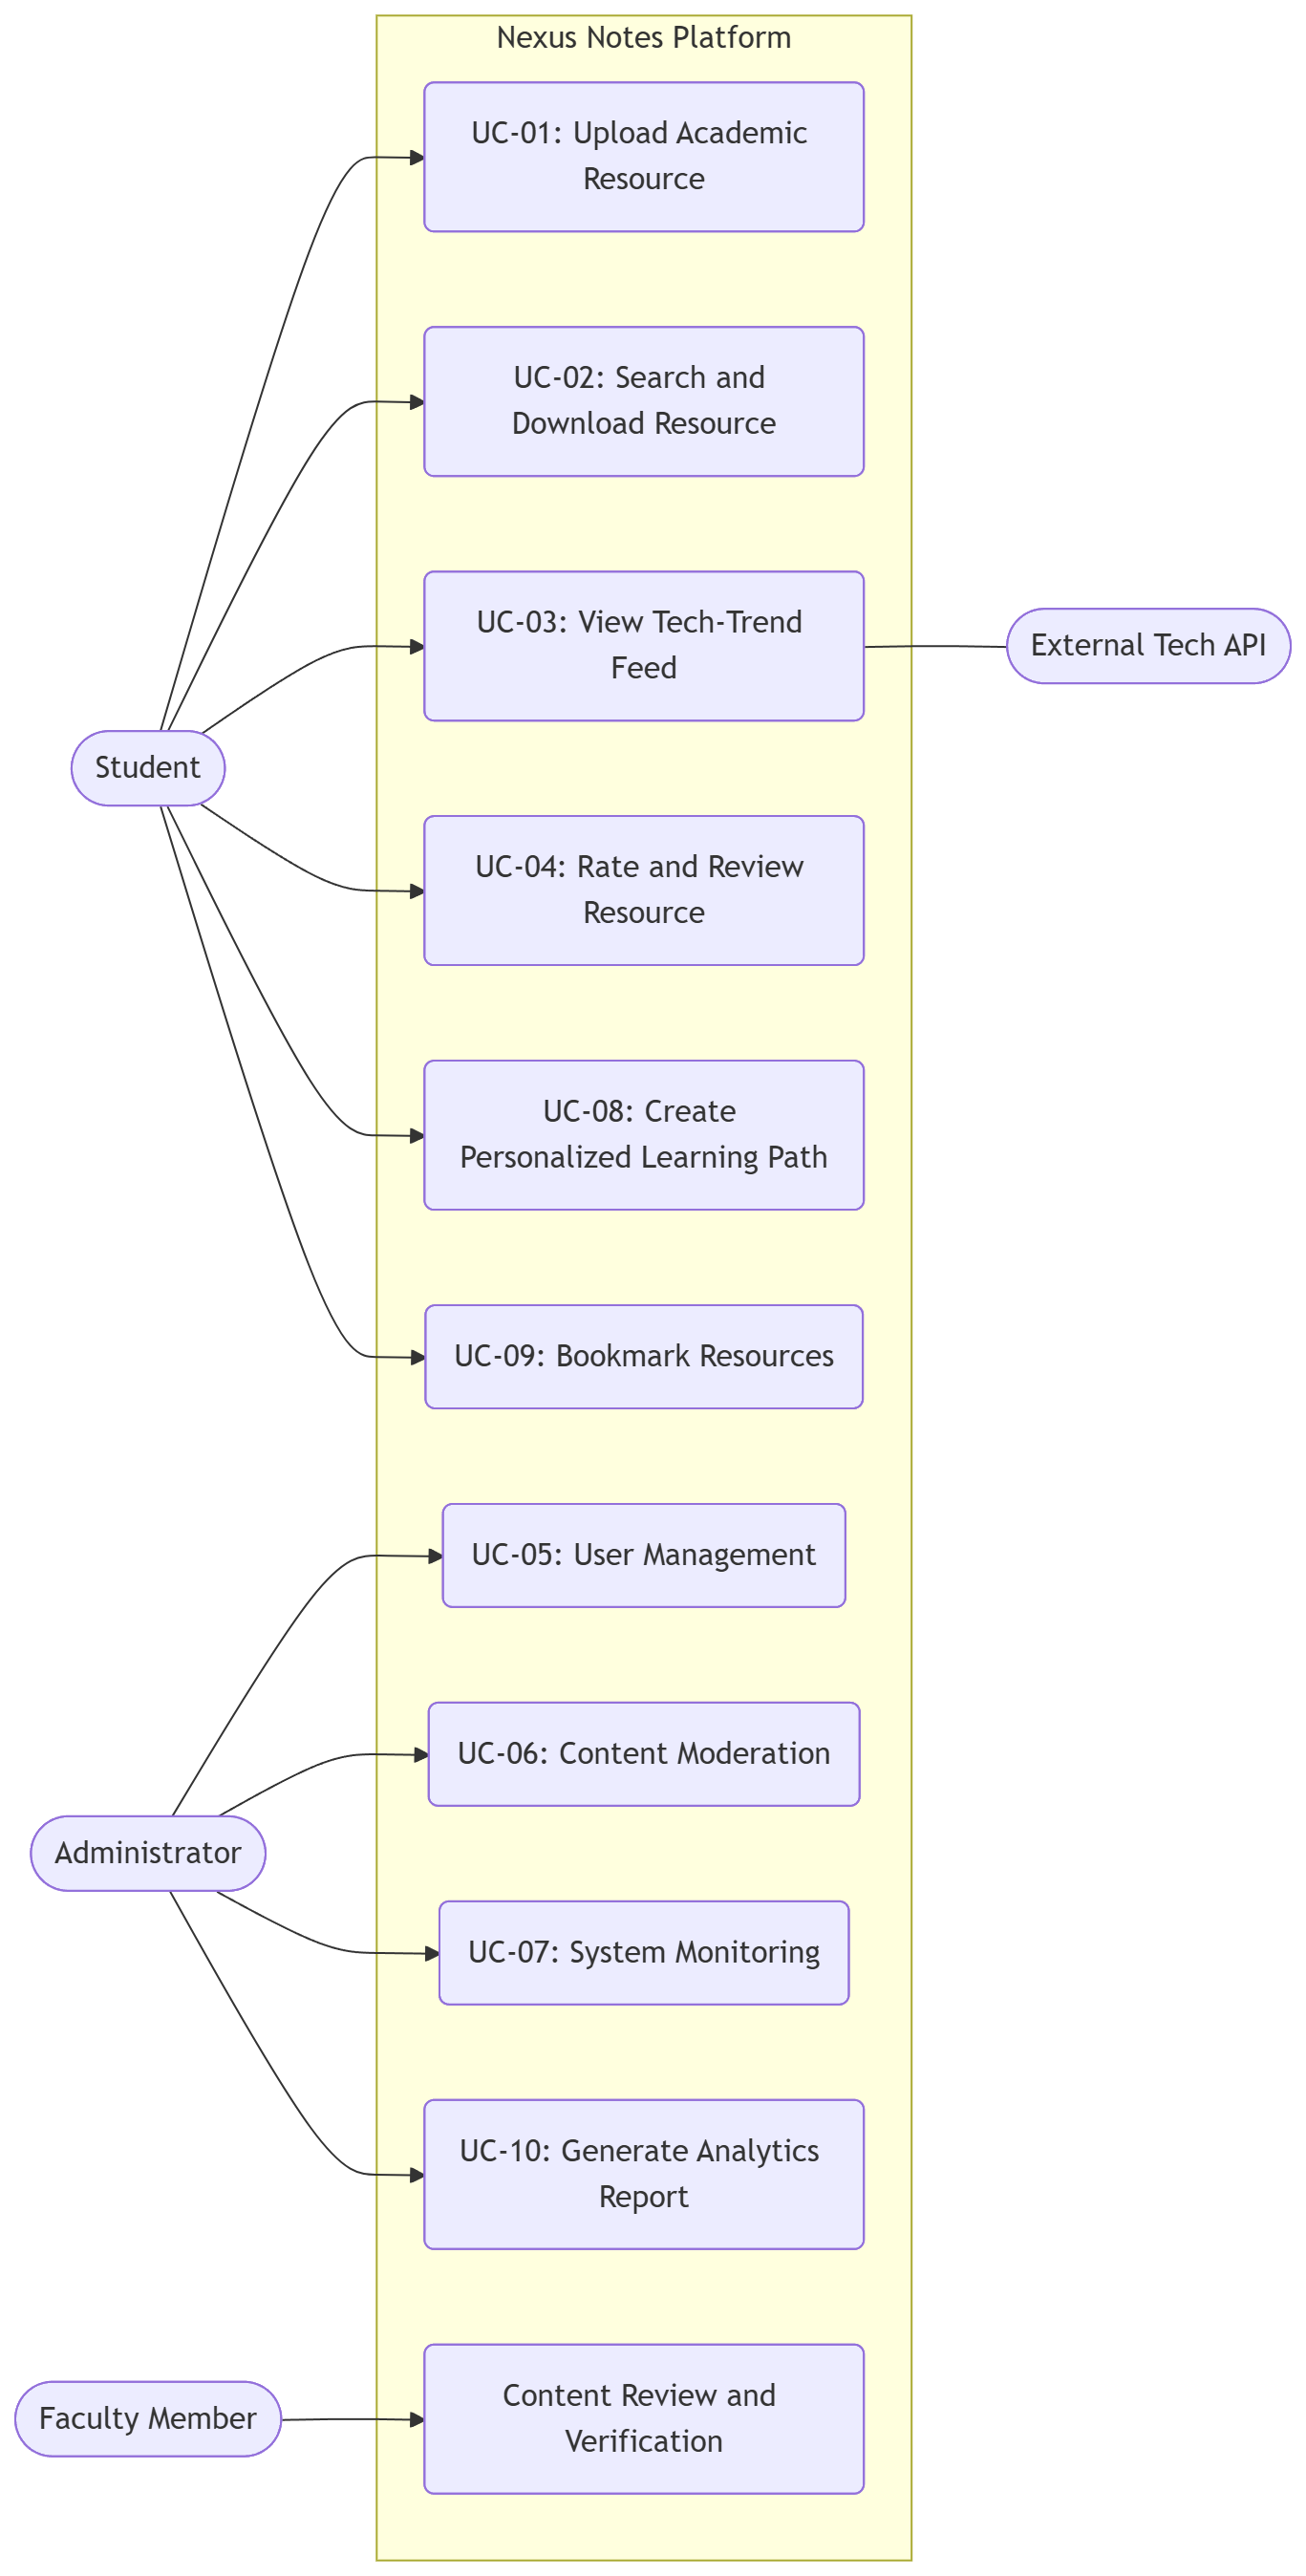
\includegraphics[width=0.8\textwidth]{mermaid-diagram-2026-03-14-094337.png}
    \caption{Use Case Diagram for Nexus Notes Platform}
    \label{fig:usecase}
\end{figure}

\subsection{Explanation}

Based on the system requirements, the primary actors in the Nexus Notes platform include the Student, Administrator, Faculty Member, and an External Tech API.

\begin{itemize}
    \item \textbf{Student:} Interacts with features such as uploading academic resources (UC-01), searching and downloading resources (UC-02), viewing the tech-trend feed (UC-03), and rating resources (UC-04).
    
    \item \textbf{Administrator:} Responsible for user management (UC-05), content moderation (UC-06), and system monitoring (UC-07).
    
    \item \textbf{Faculty Member:} Acts as a secondary user to review and verify academic content.
    
    \item \textbf{External Tech API:} A simple actor that the system interacts with to fetch real-time technological updates for the Tech-Trend Feed.
\end{itemize}

\section{Sequence Diagram: Upload Academic Resource (UC-01)}

The Sequence Diagram details the chronological step-by-step process of uploading an academic resource.

\begin{figure}[H]
    \centering
    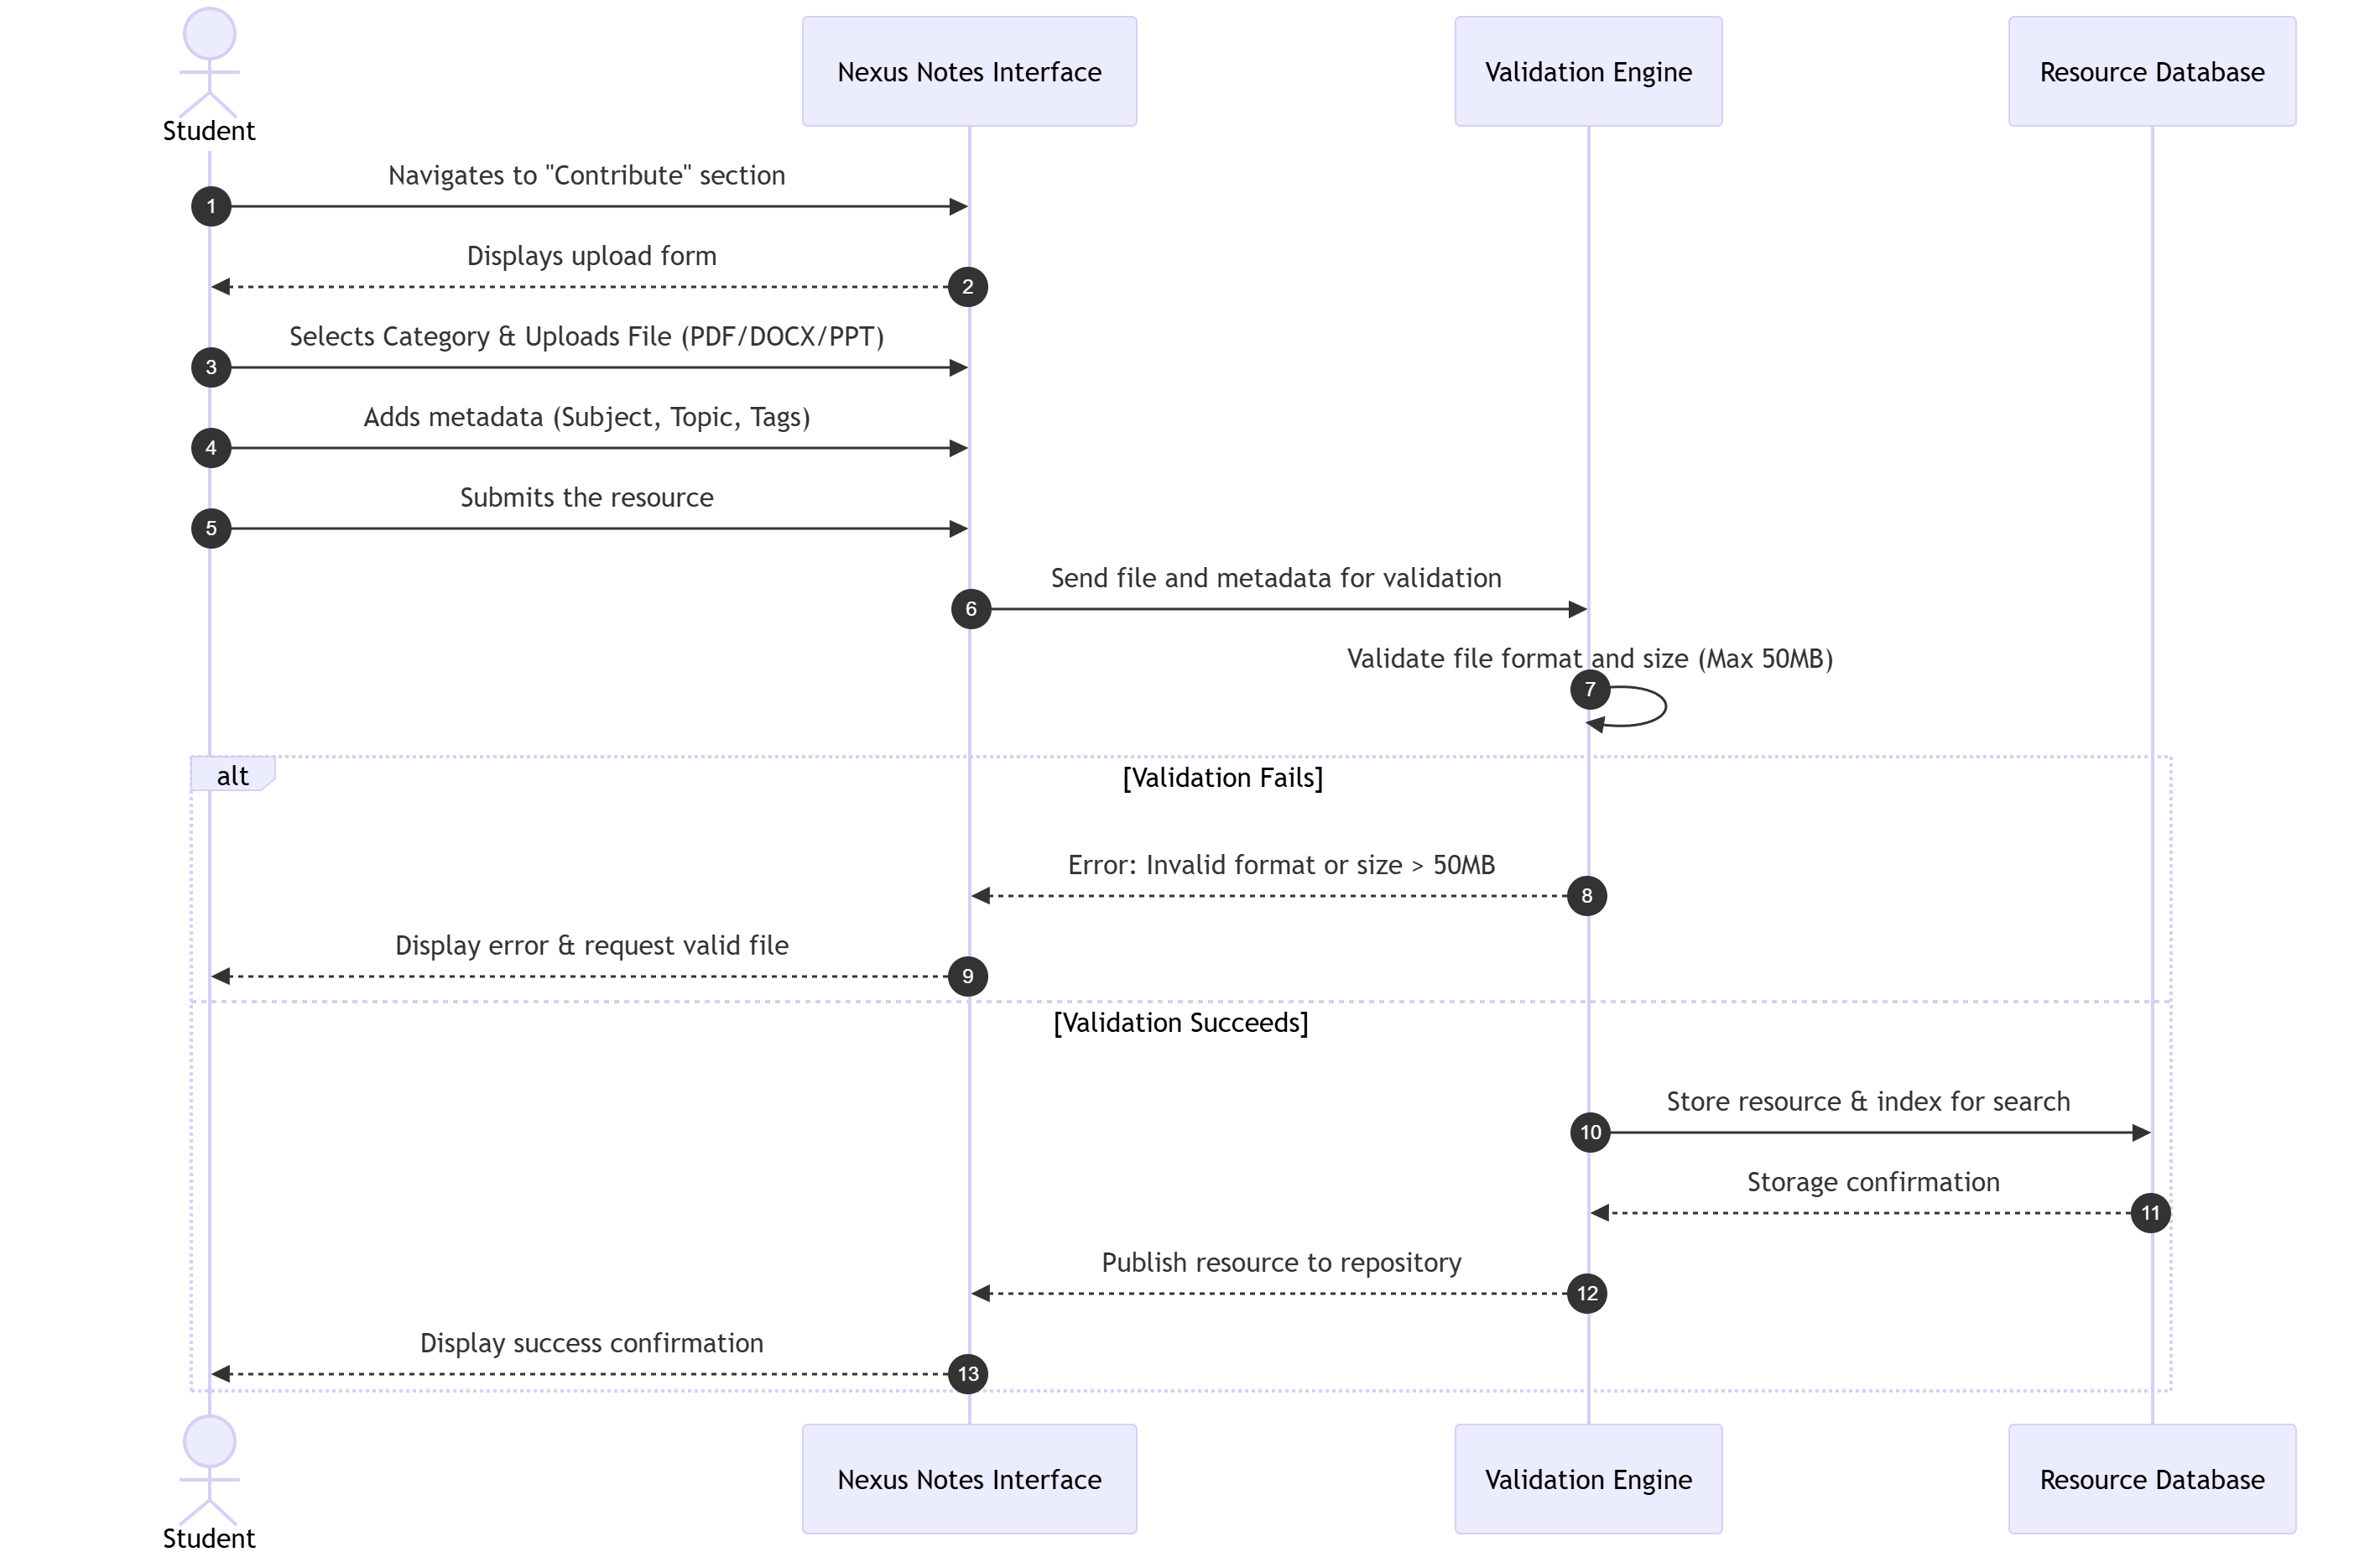
\includegraphics[width=\textwidth]{mermaid-diagram-2026-03-14-094407.png}
    \caption{Sequence Diagram for UC-01: Upload Academic Resource}
    \label{fig:sequence}
\end{figure}

\subsection{Explanation}

This diagram illustrates the normal workflow and possible exceptions for UC-01.

\begin{itemize}
    \item The student navigates to the "Contribute" section and the UI displays the upload form.
    
    \item The student selects the category, uploads a file (PDF, DOCX, PPT), adds metadata, and submits it.
    
    \item The system's validation engine checks if the file format is valid and whether the file size is under the 50MB limit.
    
    \item If validation fails (for example, due to an unsupported file type), an error message is displayed requesting a valid format.
    
    \item If validation succeeds, the resource is stored and indexed in the database, and a success confirmation is displayed to the student.
\end{itemize}

\section{Collaboration Diagram: Search and Download Resource (UC-02)}

The Collaboration Diagram (represented as a numbered communication flow) shows the structural message passing between objects during a resource search and download.

\begin{figure}[H]
    \centering
    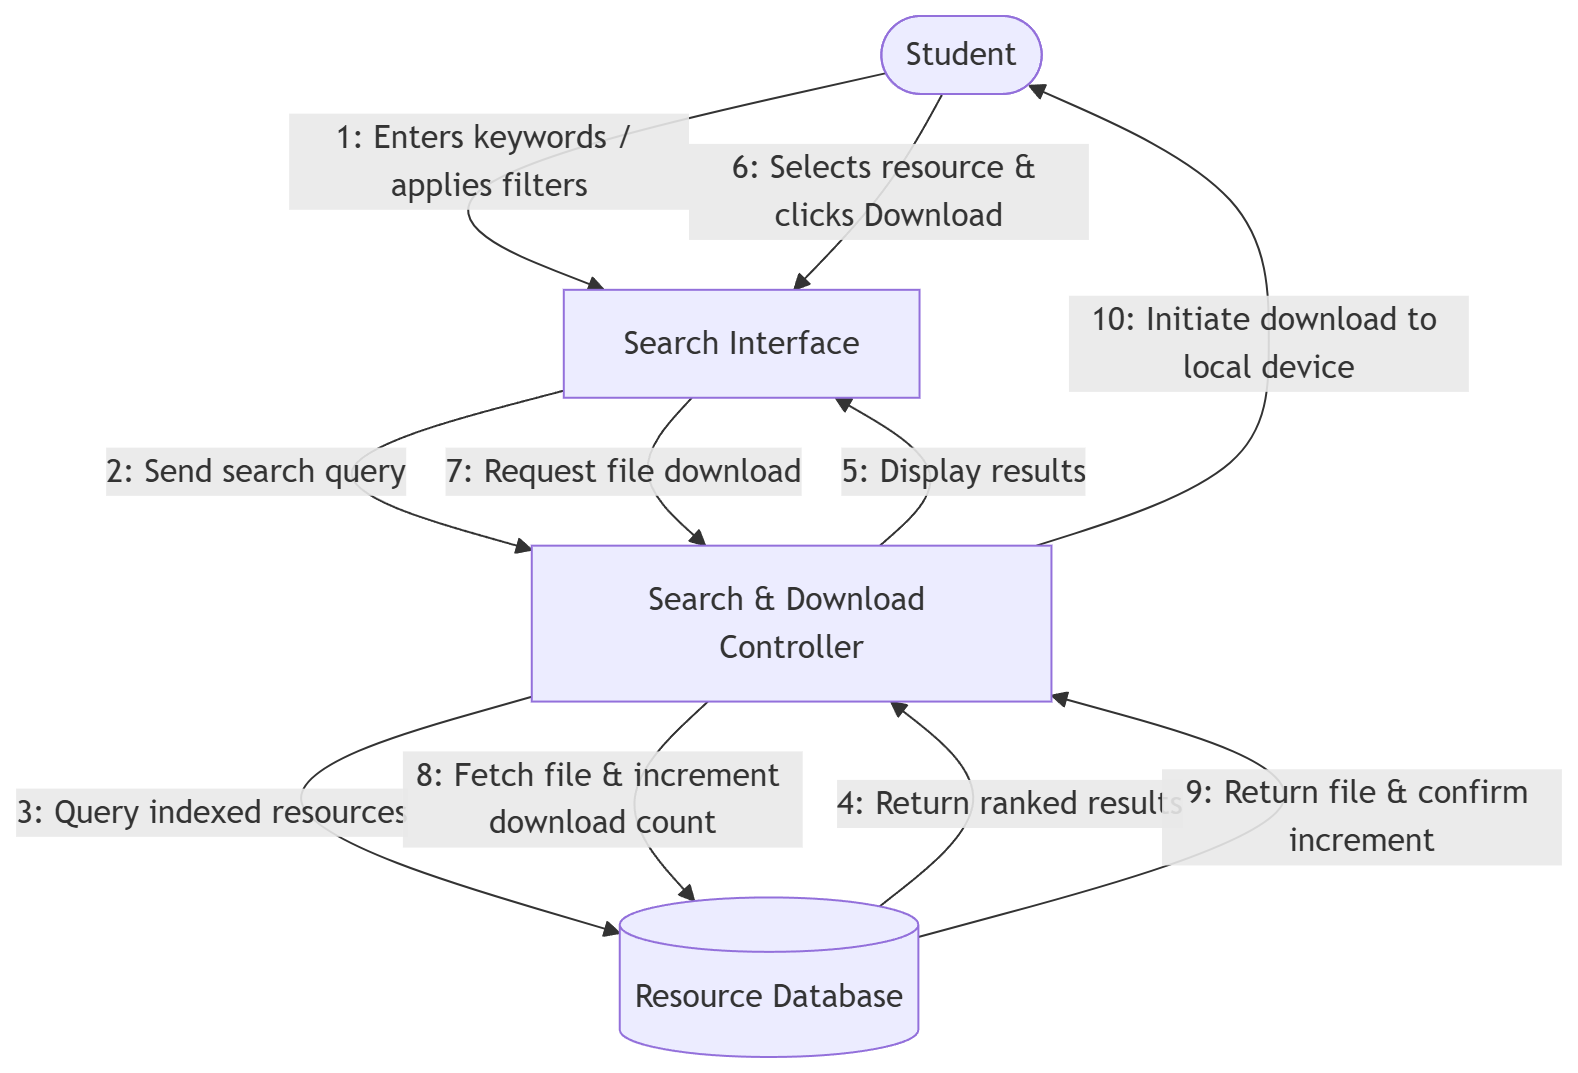
\includegraphics[width=0.9\textwidth]{mermaid-diagram-2026-03-14-094605.png}
    \caption{Collaboration Diagram for UC-02: Search and Download Resource}
    \label{fig:collaboration}
\end{figure}

\subsection{Explanation}

This diagram highlights how system components interact when a student searches for study materials using keywords or filters.

\begin{itemize}
    \item The flow begins with the student entering keywords or applying filters (such as Subject or Module) through the Search Interface.
    
    \item The query is passed to the Controller, which retrieves relevant results from the indexed Resource Database.
    
    \item The database returns ranked results based on relevance and user ratings, which are then displayed to the student.
    
    \item When the student selects a resource and clicks "Download", the system fetches the file, increments the download count in the database, and initiates the download to the student's local device.
\end{itemize}

\section{Activity Diagram: Content Moderation (UC-06)}

The Activity Diagram illustrates the control flow involved in the administrative task of moderating content.

\begin{figure}[H]
    \centering
    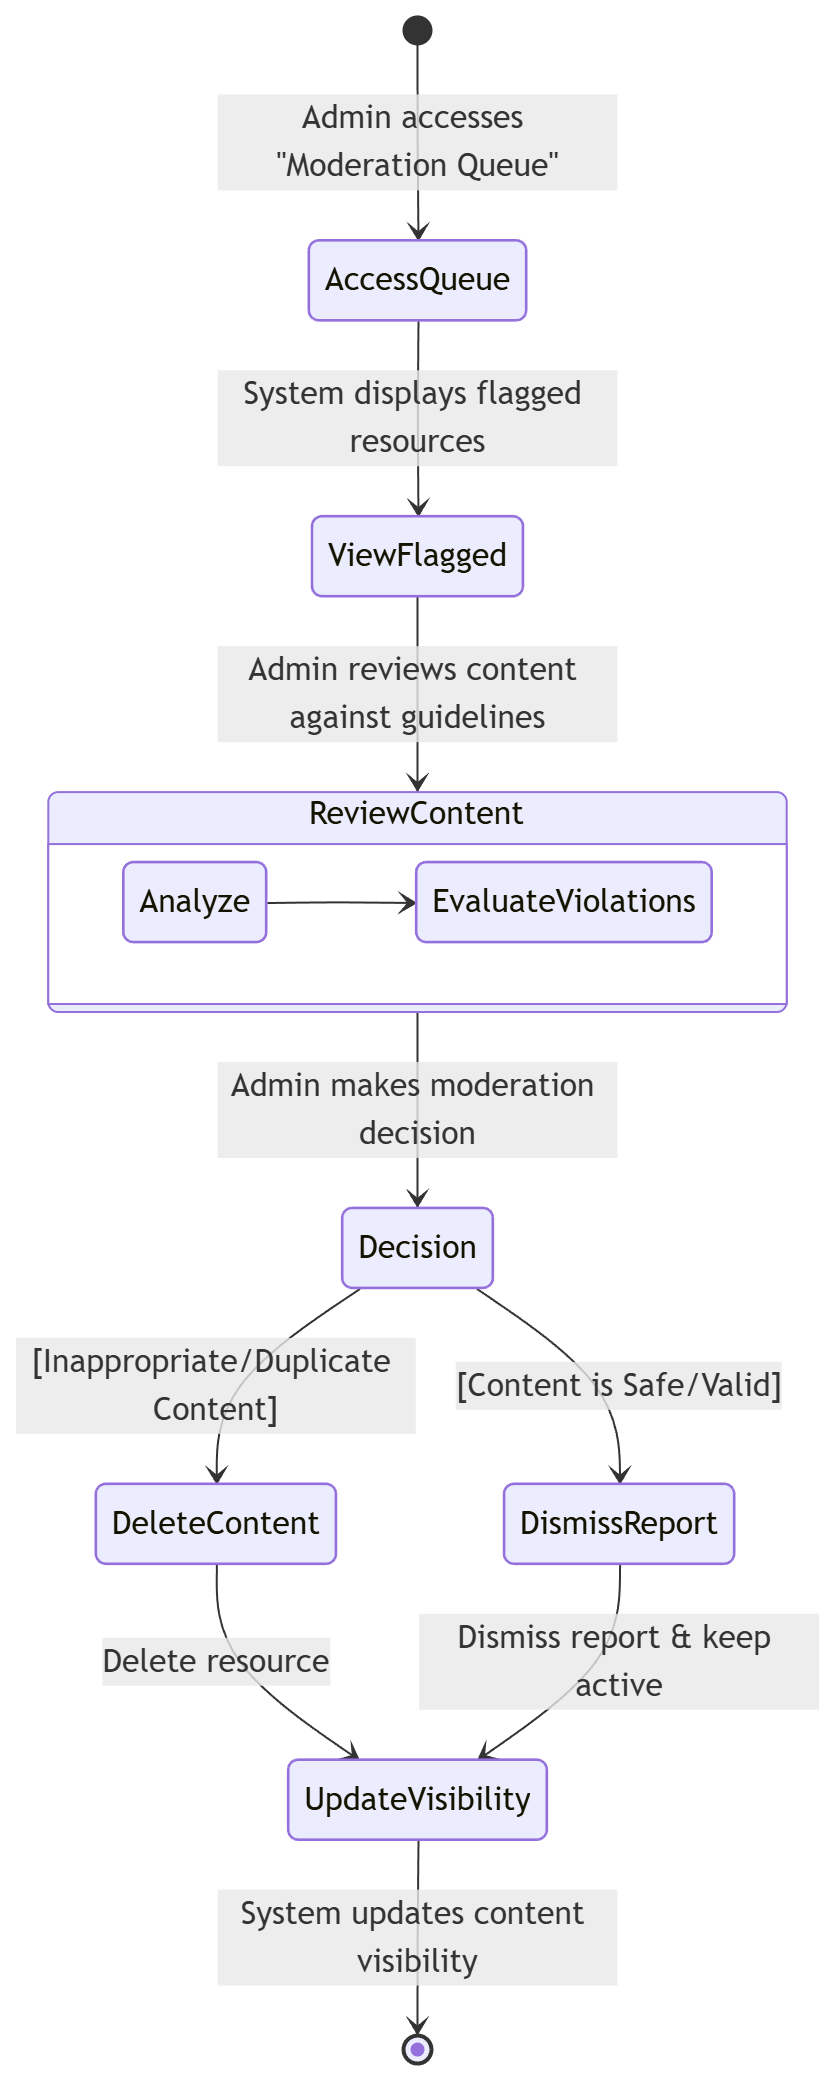
\includegraphics[width=0.6\textwidth]{mermaid-diagram-2026-03-14-094618.png}
    \caption{Activity Diagram for UC-06: Content Moderation}
    \label{fig:activity}
\end{figure}

\subsection{Explanation}

This diagram outlines the decision-making process for administrators when managing flagged content.

\begin{itemize}
    \item The Administrator accesses the Moderation Queue where the system displays flagged resources.
    
    \item The administrator reviews the content according to the platform's community guidelines.
    
    \item A moderation decision is made. If the content is inappropriate or duplicated, the administrator deletes the resource. If the report is invalid, the administrator dismisses the report and keeps the content active.
    
    \item Finally, the system updates the visibility status of the content based on the administrator's action.
\end{itemize}

\section{Software Architecture Overview}
This document details the software architecture for the Nexus Notes platform. It outlines the Logical View, Component View, and Deployment View using Unified Modeling Language (UML) diagrams. The architecture is built around a modern MERN stack (MongoDB, Express.js, React, Node.js) to support a robust, student-centric academic resource ecosystem.

\section{Logical View: Class Diagram}
The Class Diagram maps the object-oriented structure of the Nexus Notes system, defining the core entities, their attributes, methods, and relationships.

\begin{figure}[H]
    \centering
    % Added max height and keepaspectratio to prevent overflow
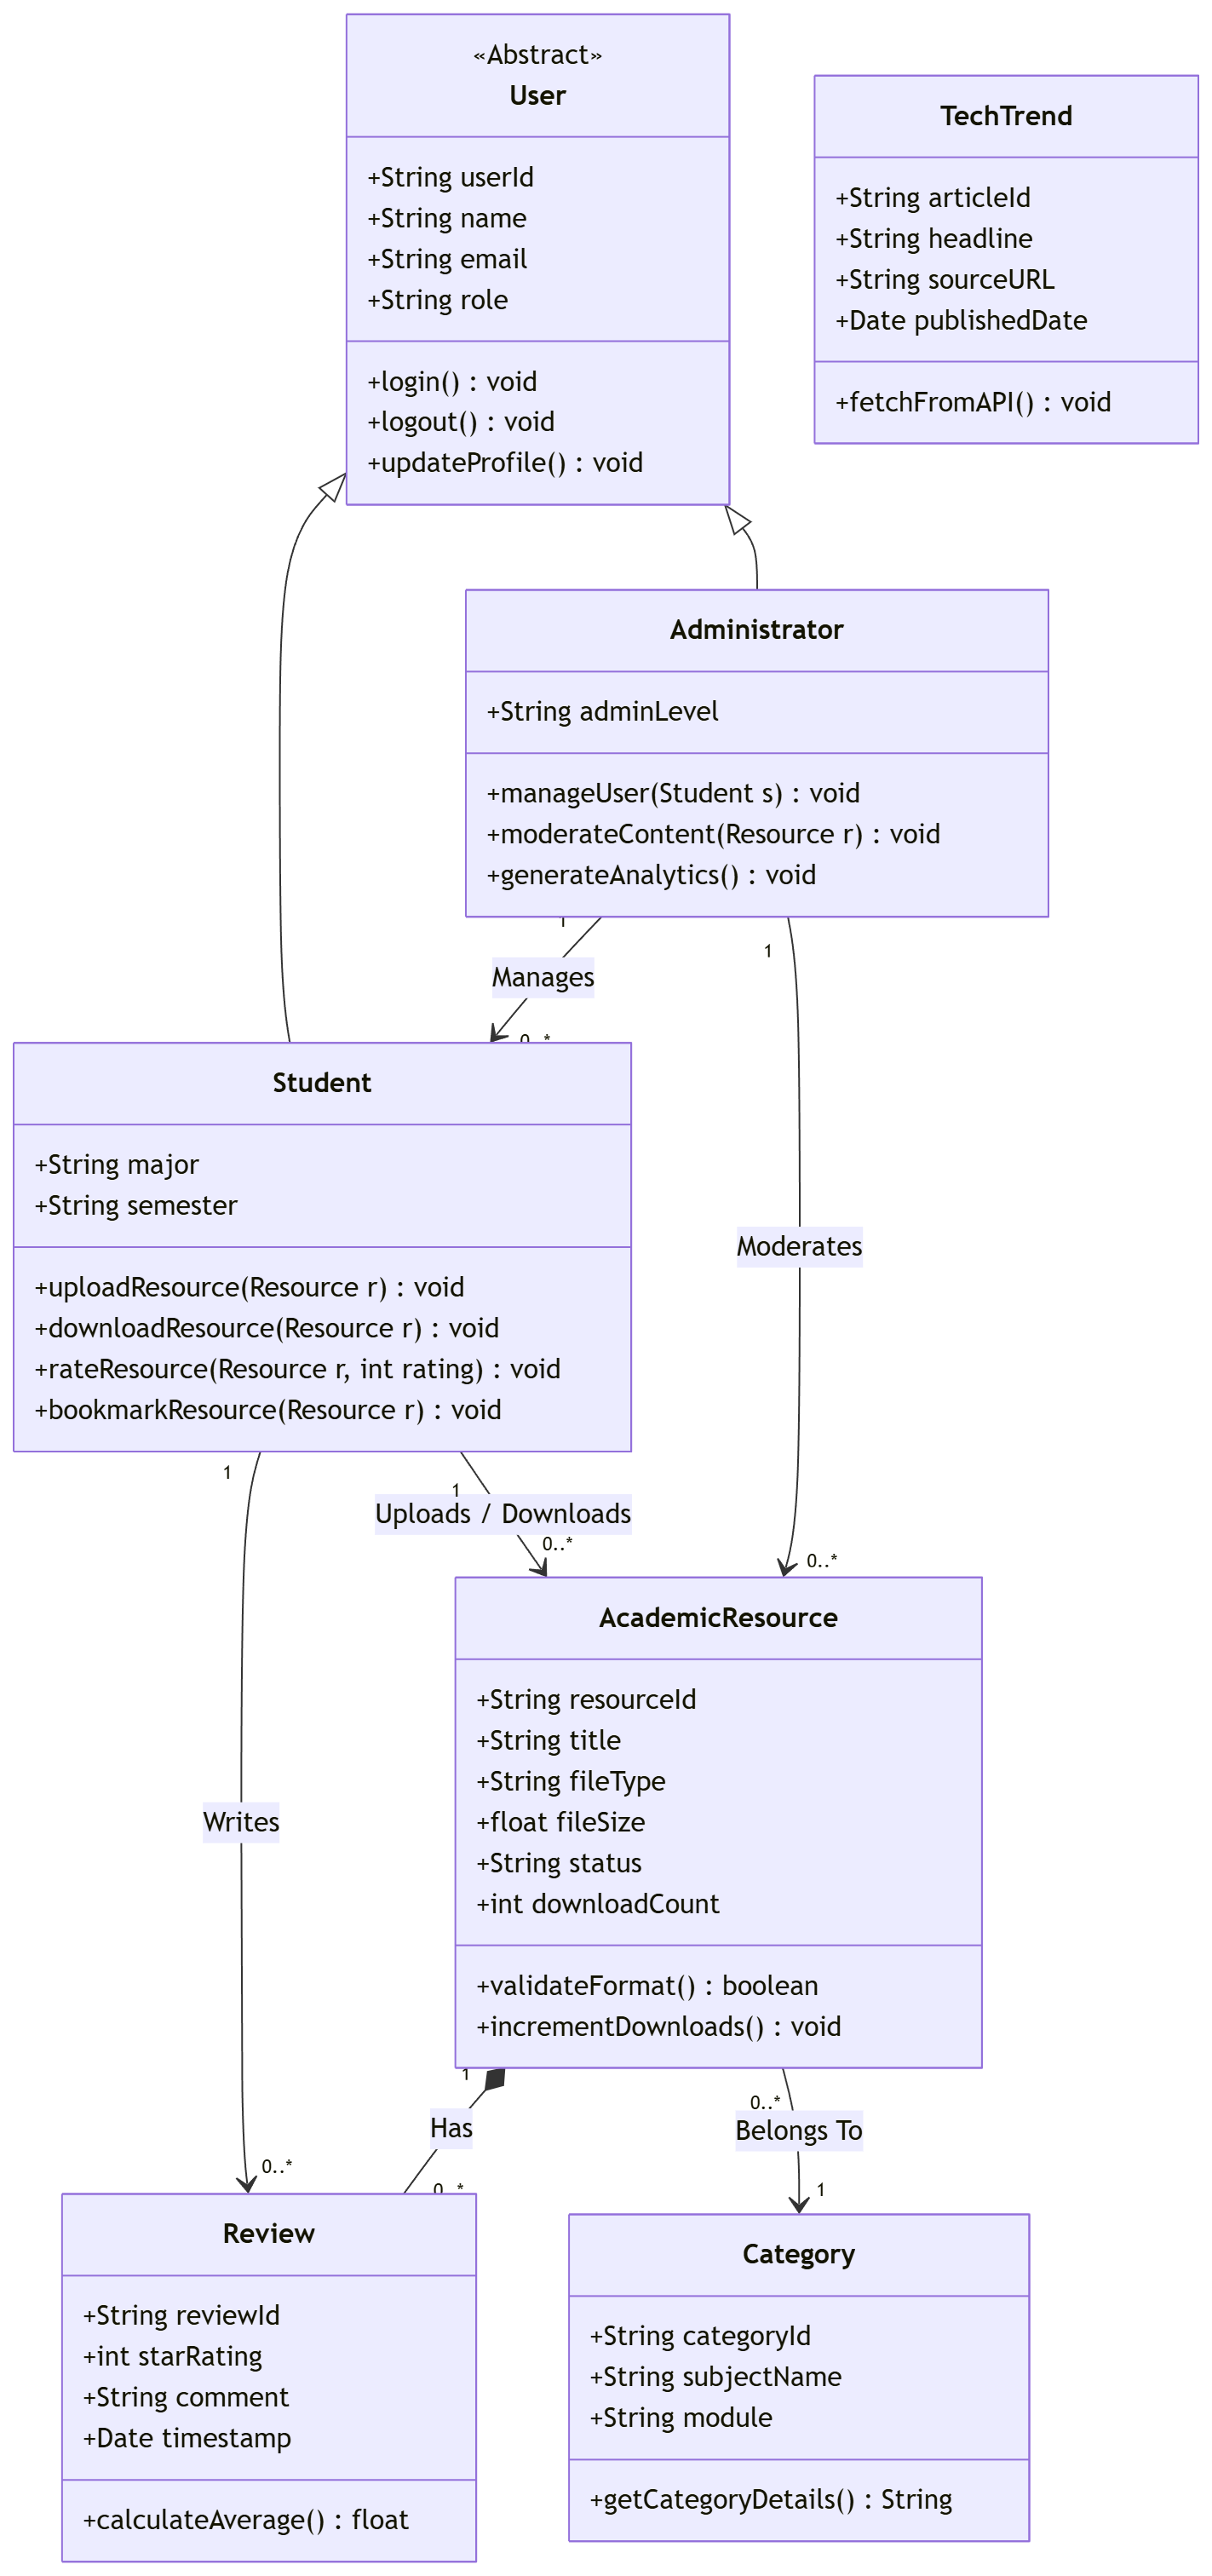
\includegraphics[width=0.6\textwidth]{class.png}
    \caption{Logical View: Class Diagram}
    \label{fig:class}
\end{figure}

\subsection{Explanation}
The system's data structure revolves around the primary stakeholders—the students—and the resources they interact with.
\begin{itemize}
    \item \textbf{User Hierarchy:} The abstract \texttt{User} class provides base attributes (ID, name, email) and authentication methods. The \texttt{Student} class inherits from this base, adding specific behaviors like uploading, downloading, and bookmarking resources. The \texttt{Administrator} class also inherits from \texttt{User} and handles moderation and user management.
    \item \textbf{AcademicResource \& Category:} The \texttt{AcademicResource} class encapsulates file metadata (size, format, download count) and lifecycle methods. It maintains a many-to-one relationship with the \texttt{Category} class, ensuring all materials are strictly organized by subject and module.
    \item \textbf{Review System:} The \texttt{Review} class acts as a transactional entity linked to \texttt{AcademicResource}, storing star ratings and comments left by students to drive the platform's intelligent ranking system.
    \item \textbf{TechTrend:} A standalone entity that models the data fetched from the external APIs to keep students informed on emerging technologies.
\end{itemize}

\section{Logical View: Statechart Diagram}
The Statechart Diagram illustrates the lifecycle and varying states of an \texttt{AcademicResource} within the Nexus Notes platform.

\begin{figure}[H]
    \centering
    % Added max height and keepaspectratio to prevent overflow
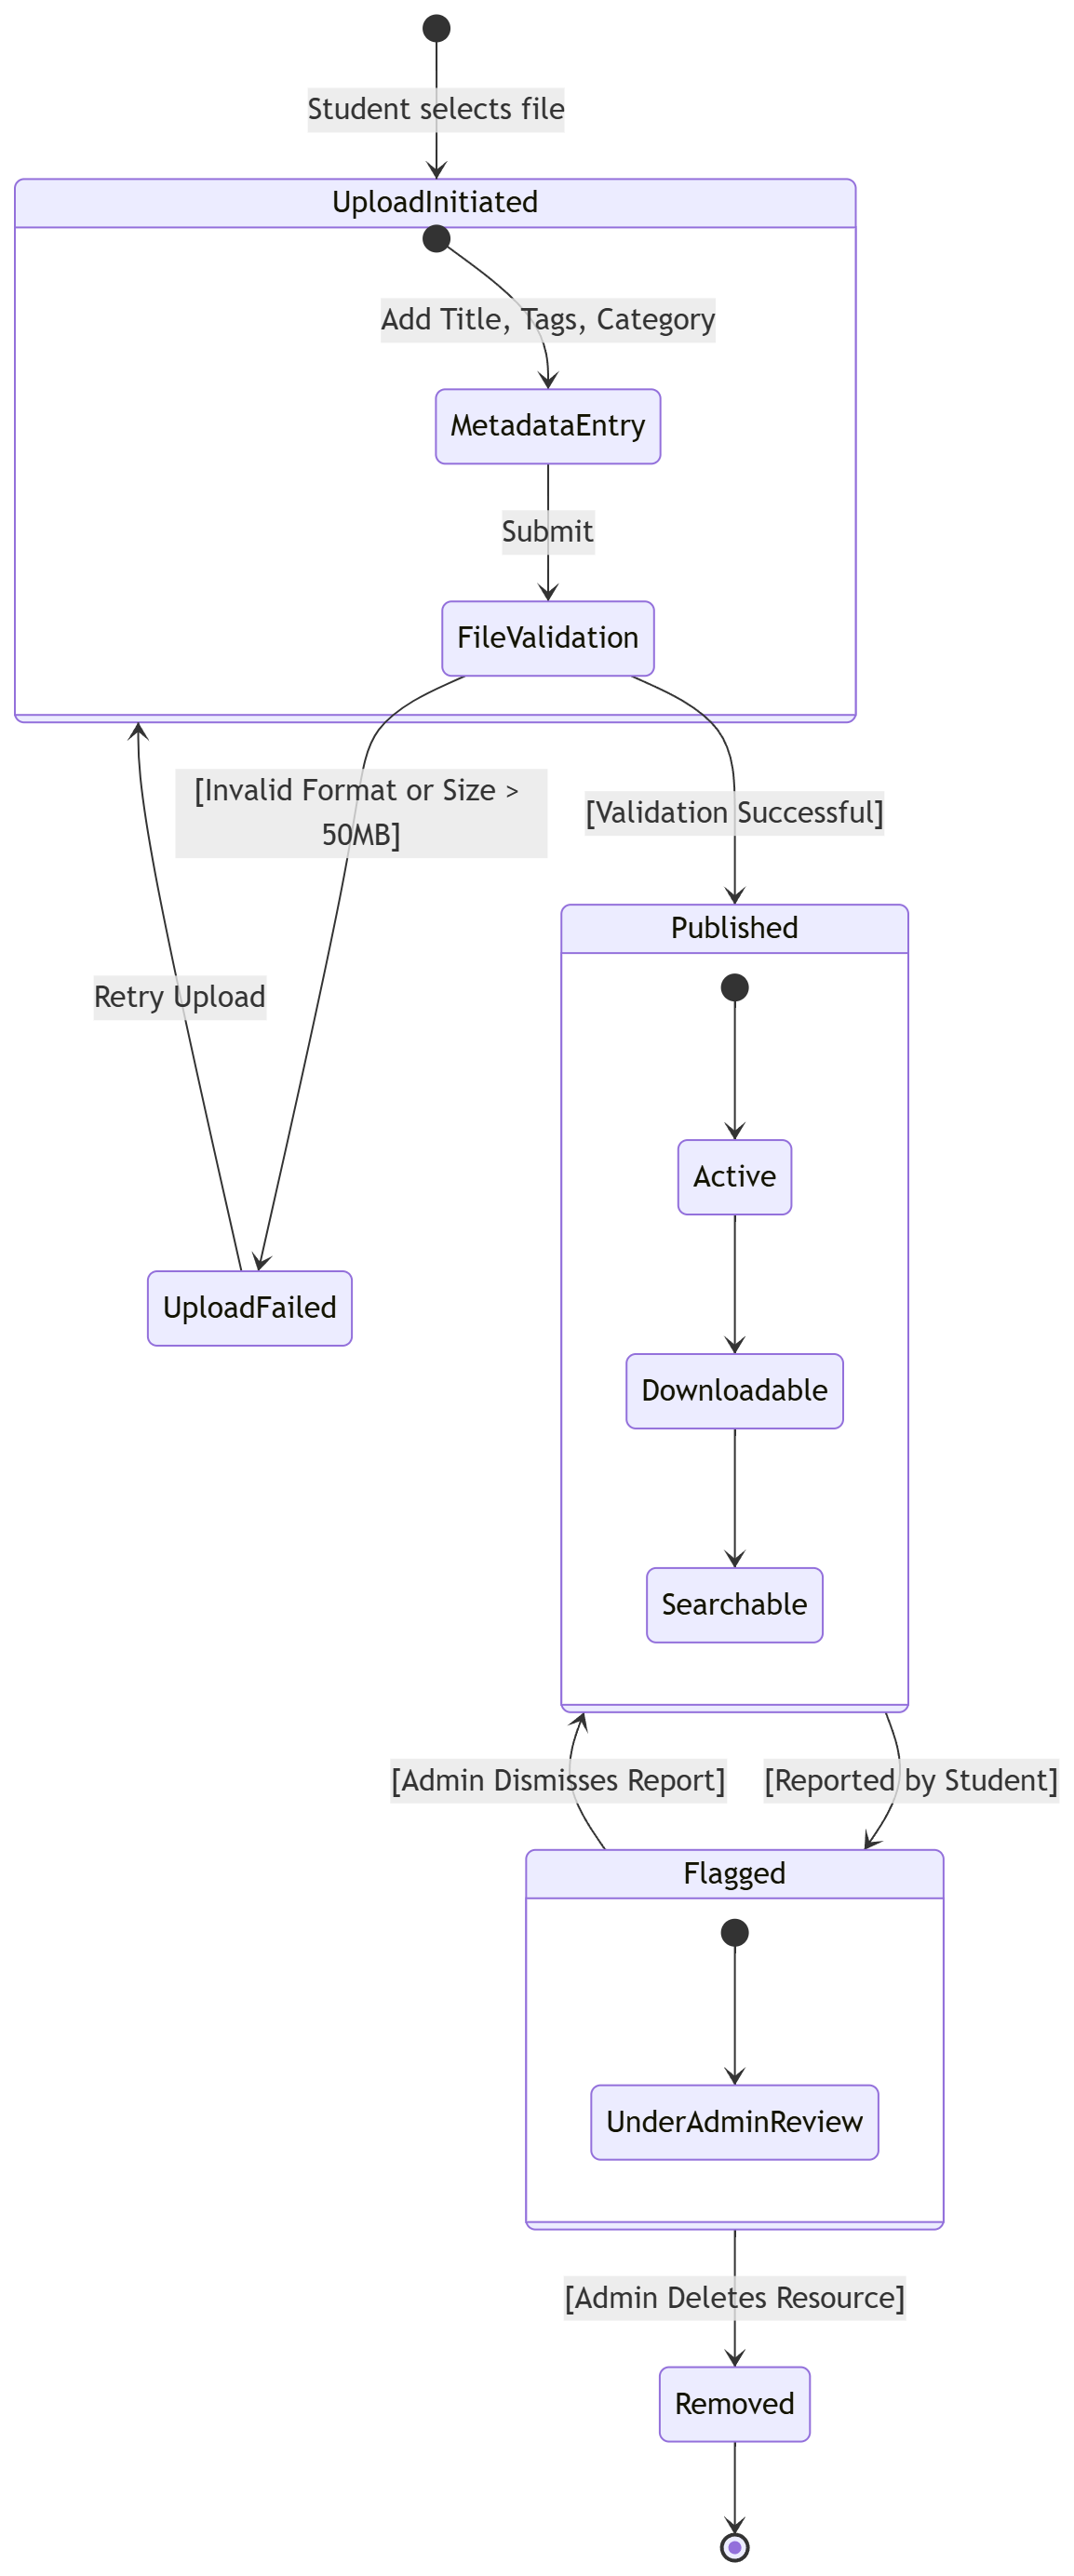
\includegraphics[width=0.6\textwidth]{statechart.png}
    \caption{Logical View: Statechart Diagram}
    \label{fig:statechart}
\end{figure}

\subsection{Explanation}
This diagram tracks the dynamic behavior of an academic file from the moment a student initiates an upload.
\begin{itemize}
    \item \textbf{Upload \& Validation:} The process begins in the \texttt{UploadInitiated} state. Once the student inputs the required metadata, the system transitions to \texttt{FileValidation}. If the file exceeds 50MB or uses an unsupported format, it enters the \texttt{UploadFailed} state, prompting a retry.
    \item \textbf{Active State:} Upon successful validation, the resource transitions to \texttt{Published}. Here, it simultaneously becomes \texttt{Downloadable} and \texttt{Searchable} for the student body.
    \item \textbf{Moderation Flow:} If a student reports the content, the resource shifts to the \texttt{Flagged} state, triggering an \texttt{UnderAdminReview} sub-state. Depending on the administrator's evaluation, it is either returned to the \texttt{Published} state or permanently transitioned to \texttt{Removed}.
\end{itemize}

\section{Component View: Component Diagram}
The Component Diagram details the modular structure of the Nexus Notes software application, mapped specifically to the MERN stack environment.

\begin{figure}[H]
    \centering
    % Added max height and keepaspectratio to prevent overflow
    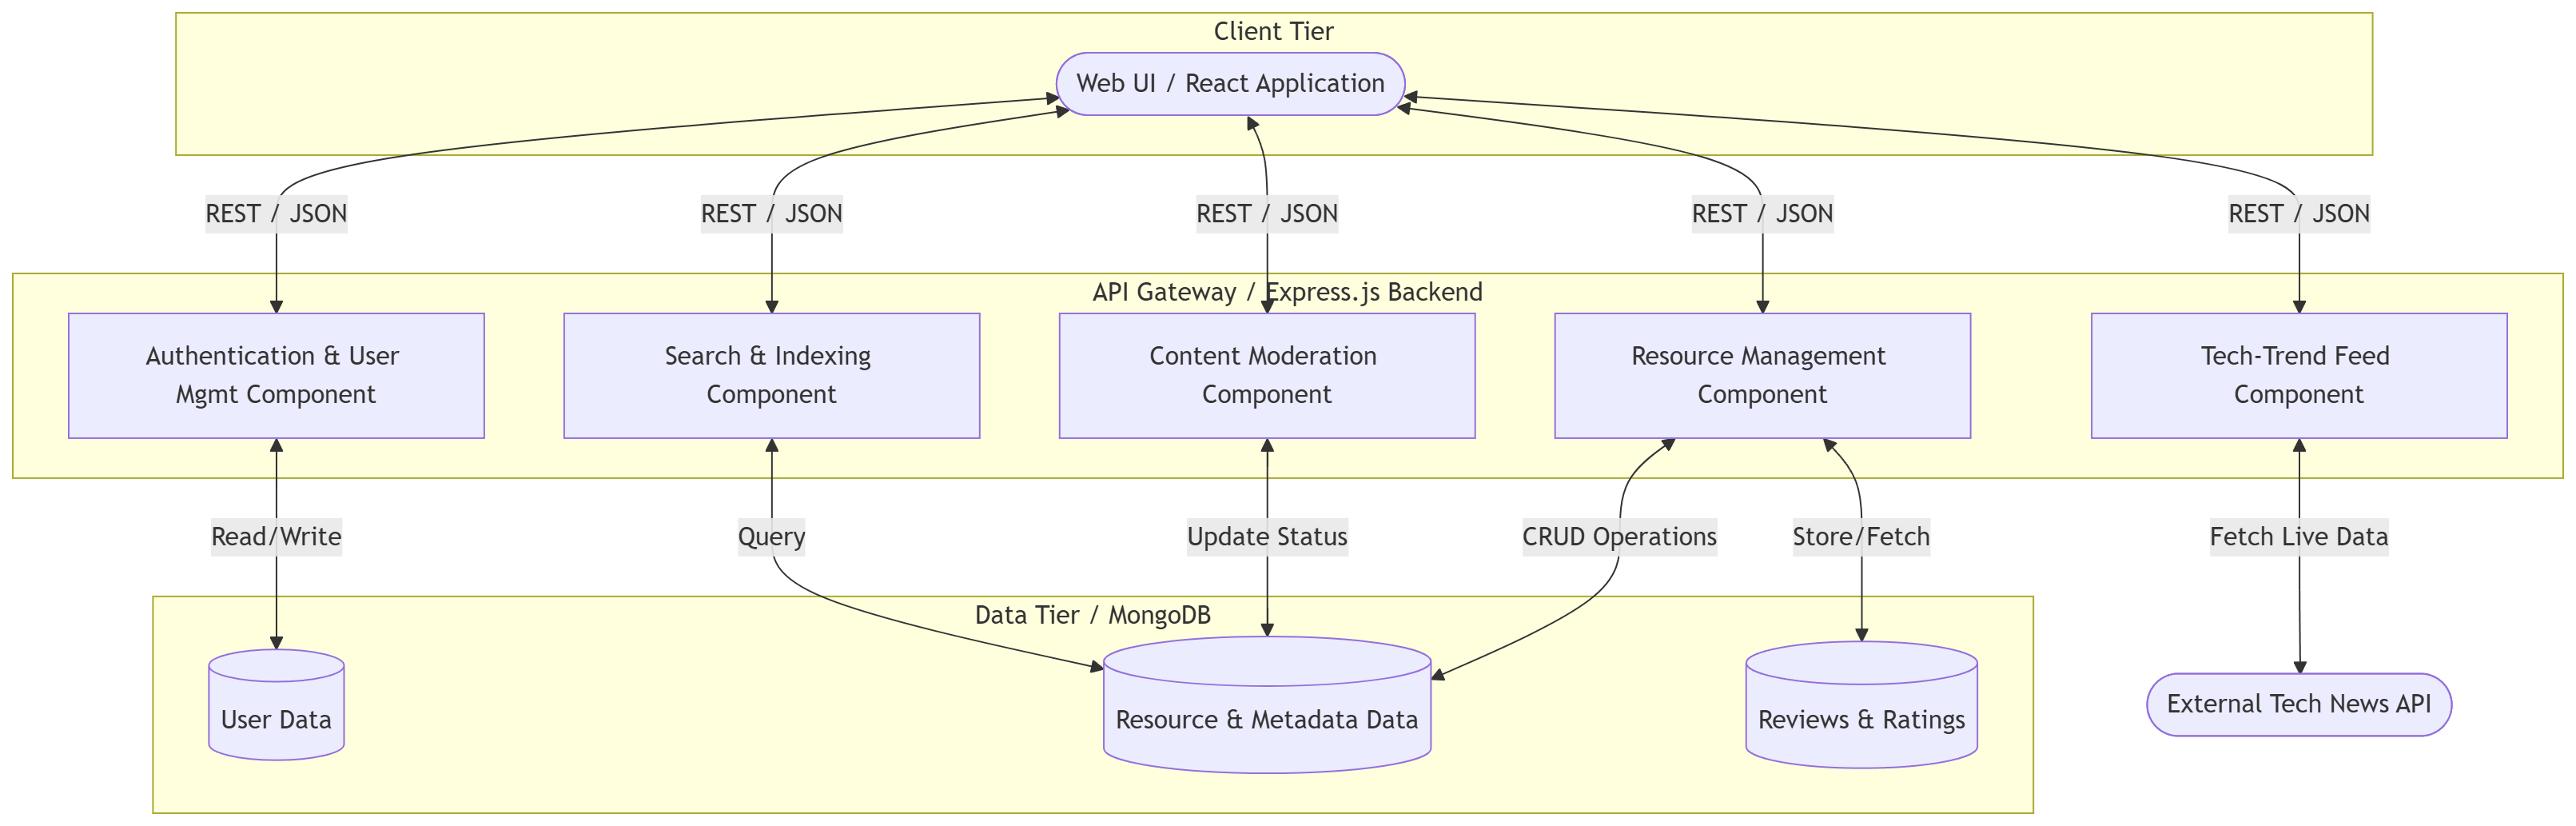
\includegraphics[width=\textwidth, height=0.4\textheight, keepaspectratio]{component.png}
    \caption{Component View: Component Diagram}
    \label{fig:component}
\end{figure}

\subsection{Explanation}
The system is divided into three highly decoupled tiers to ensure maintainability and scalability.
\begin{itemize}
    \item \textbf{Client Tier:} The Web UI is a Single Page Application (SPA) built with React. It handles all user interactions and dynamic rendering of dashboards.
    \item \textbf{Application Tier (API Gateway):} The Node.js and Express.js backend serves as the bridge. It is composed of independent functional modules: Authentication, Resource Management, Search \& Indexing, Content Moderation, and the Tech-Trend Feed component (which communicates securely with external APIs).
    \item \textbf{Data Tier:} The persistent storage is handled by MongoDB. Data is logically separated into \texttt{User Data}, \texttt{Resource \& Metadata Data}, and \texttt{Reviews \& Ratings} databases to optimize query times during complex searches.
\end{itemize}

\section{Deployment View: Deployment Diagram}
The Deployment Diagram visualizes the physical execution architecture and how software artifacts are distributed across hardware nodes.

\begin{figure}[H]
    \centering
    % Added max height and keepaspectratio to prevent overflow
    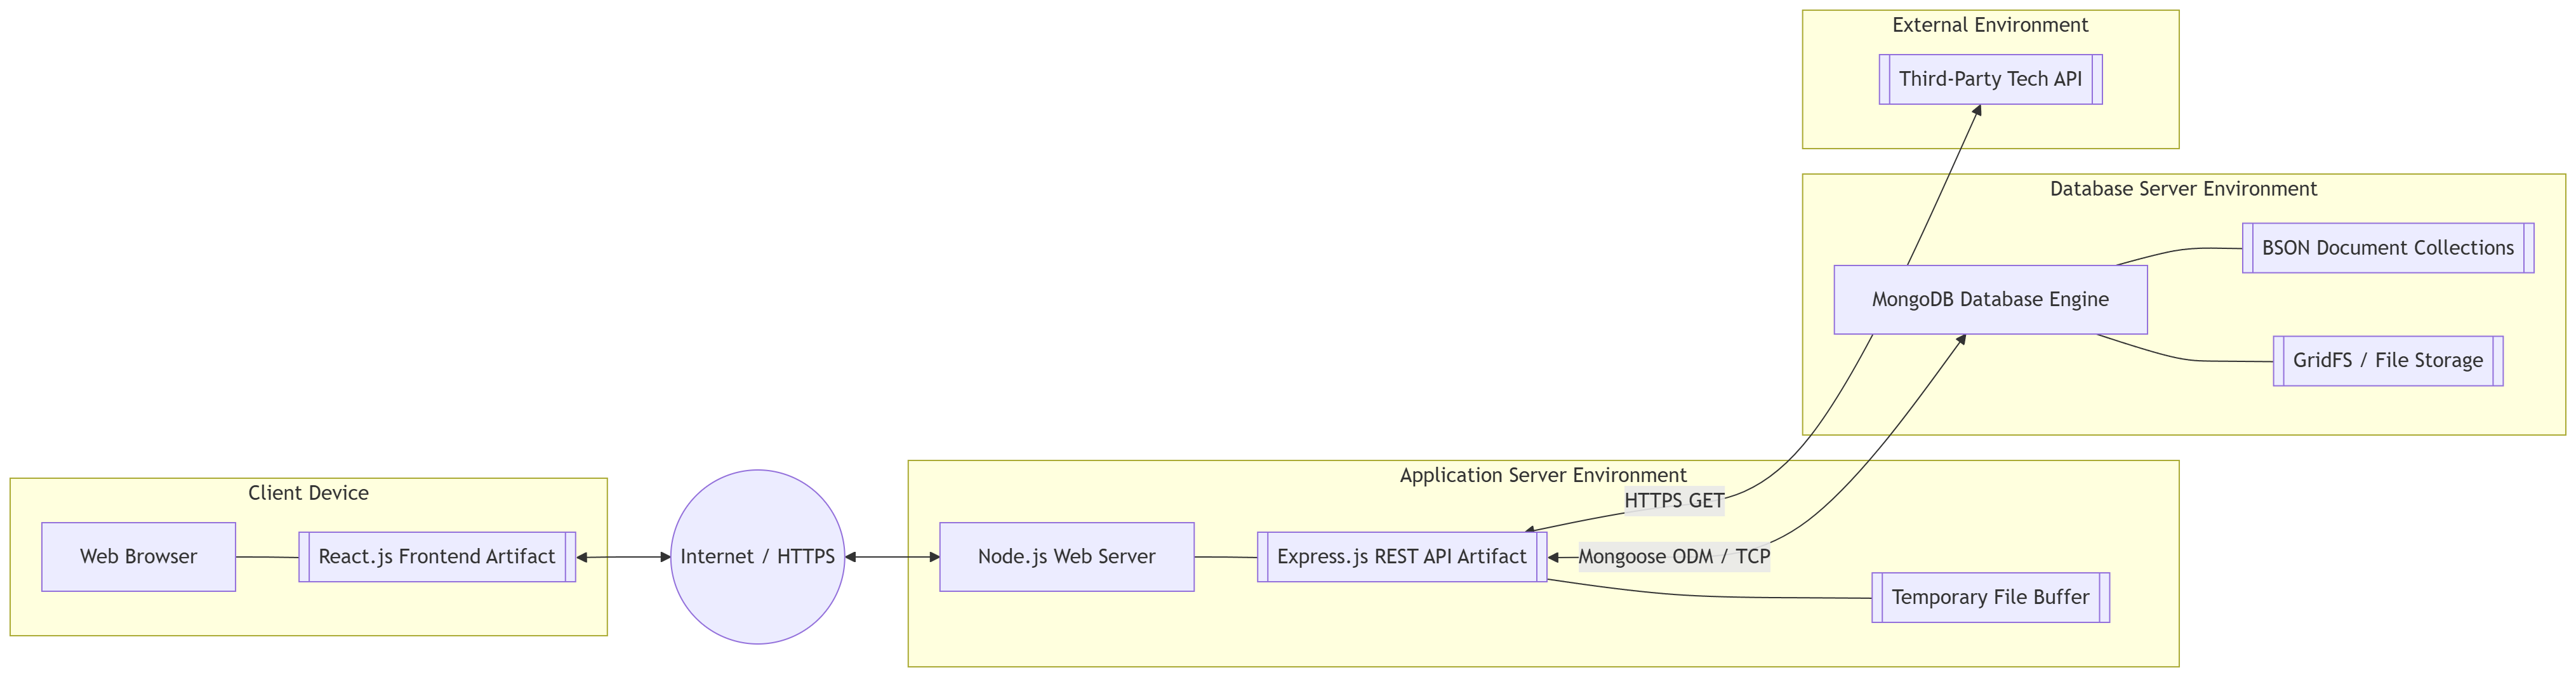
\includegraphics[width=0.9\textwidth, height=0.4\textheight, keepaspectratio]{deployment.png}
    \caption{Deployment View: Deployment Diagram}
    \label{fig:deployment}
\end{figure}

\subsection{Explanation}
The deployment topology outlines how students access the system and how the servers process those requests.
\begin{itemize}
    \item \textbf{Client Device:} Represents the student's hardware (laptop, tablet, or smartphone). The execution environment is a standard Web Browser running the compiled React.js frontend artifact.
    \item \textbf{Application Server Environment:} A cloud-hosted Node.js web server running the Express.js REST API. This node handles all business logic, routing, and temporary file buffering during uploads.
    \item \textbf{Database Server Environment:} A dedicated MongoDB server cluster. It utilizes BSON document collections for highly flexible metadata storage and GridFS for chunking and storing the actual academic resource files (PDFs, PPTs) natively within the database structure.
    \item \textbf{External Environment:} Represents the third-party Tech API servers, accessed asynchronously over HTTPS by the application server to populate the student dashboard.
\end{itemize}

\end{document}
